% The title frame of colloquium_on_the_machine.tex, which inputs this file.
% The title page is the course poster on white: the poster's statue
% (figures/poster/make_title_statue.py) beside the theme's title block, whose
% last line is broken in two so it ends left of the statue. The braces keep
% the white page and the dark text on this one frame.
{%
\setbeamercolor{title}{fg=black}
\setbeamercolor{author}{fg=DHBWgray}
\setbeamercolor{institute}{fg=DHBWgray}
\usebackgroundtemplate{%
  \begin{tikzpicture}
    \useasboundingbox (0,0) rectangle (\paperwidth,\paperheight);
    \fill[white] (0,0) rectangle (\paperwidth,\paperheight);
    \node[anchor=south east,inner sep=0pt] at (\paperwidth,3mm)
      {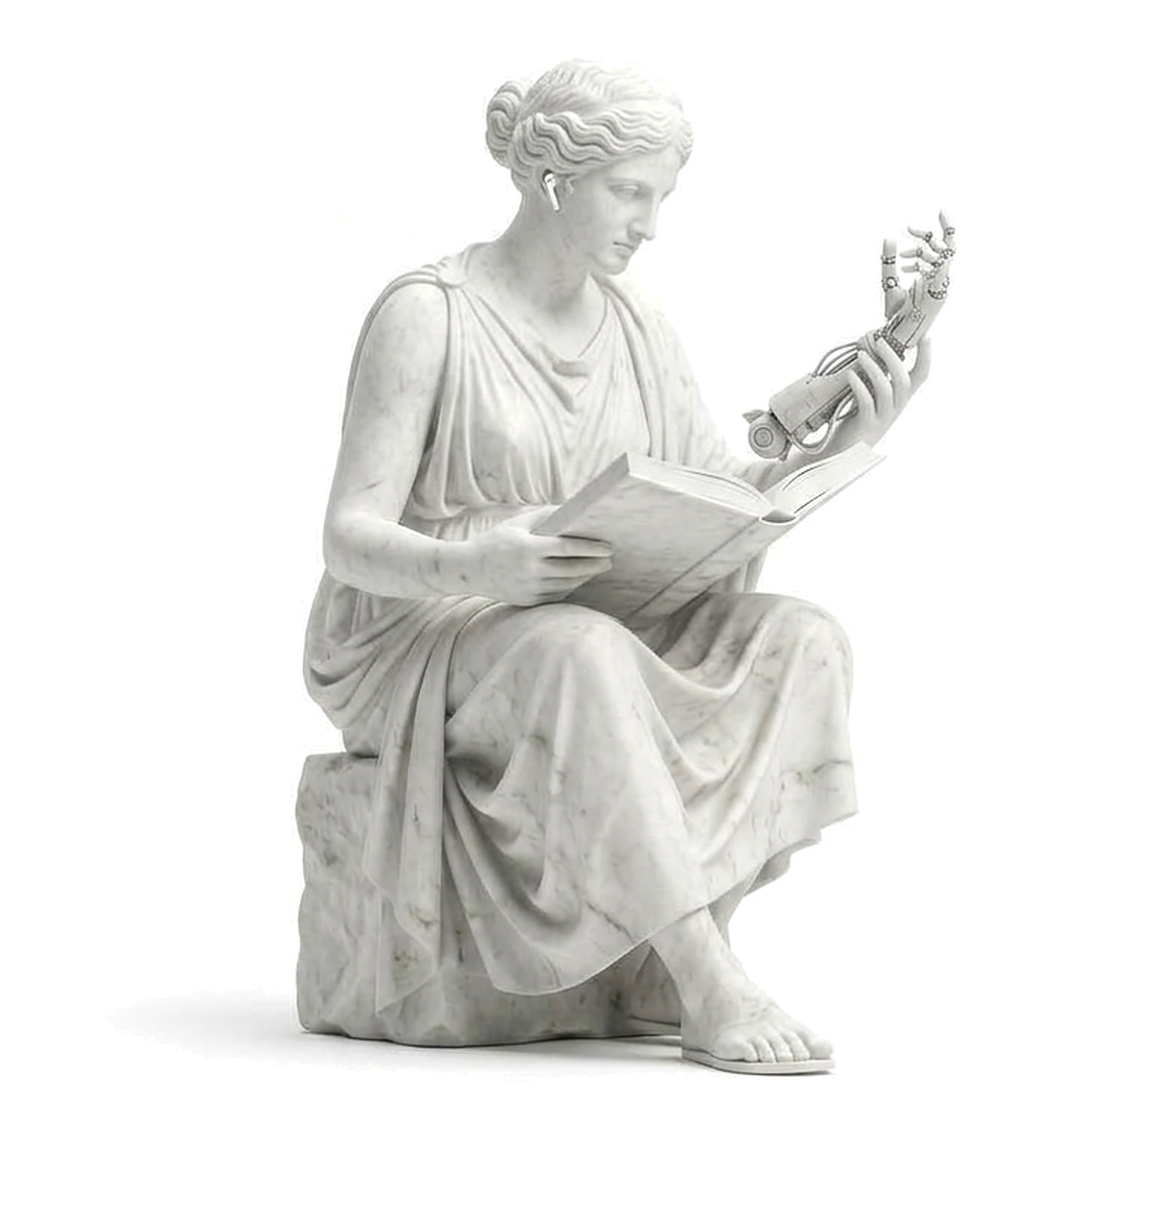
\includegraphics[height=0.95\paperheight]{title_statue}};
    \node[anchor=south east,inner sep=0pt,font=\tiny,text=DHBWgray]
      at (\paperwidth-3mm,3mm) {Image created with Google Gemini};
  \end{tikzpicture}}
\setbeamertemplate{title page}{%
  \vskip2mm%
  {\small\usebeamercolor[fg]{institute}\insertinstitute}\par%
  \vfill
  {\color{DHBWred}\rule{0.16\paperwidth}{2pt}}\par\vskip0.8em%
  {\usebeamerfont{title}\usebeamercolor[fg]{title}\inserttitle\par}%
  \vskip3em%
  {\normalsize\usebeamercolor[fg]{author}\insertauthor\par
    \vskip0.3em\printbookversion\par}%
  \vfill
}
\begin{frame}[plain]
  \titlepage
\end{frame}}
